\documentclass[12pt, a4paper]{book}

\usepackage[T1]{fontenc}
\usepackage[utf8]{inputenc}
\usepackage[charter, cal=cmcal]{mathdesign}
\usepackage[scaled=0.92]{helvet}
\usepackage{geometry}
\geometry{a4paper, top=30mm, bottom=30mm, inner=32mm, outer=25mm, marginparwidth=18mm}

\usepackage{amsmath, amsthm}
\usepackage[version=4]{mhchem}
\usepackage{graphicx}
\usepackage{xcolor}
\usepackage{tikz}
\usetikzlibrary{arrows.meta, shapes.geometric, positioning, calc, backgrounds}
\usepackage{pgfplots}
\pgfplotsset{compat=1.18}
\usepackage{tcolorbox}
\tcbuselibrary{skins, breakable, theorems}
\usepackage{titlesec}
\usepackage{fancyhdr}
\usepackage{enumitem}
\usepackage{booktabs}
\usepackage{array}
\usepackage{parskip}
\usepackage{siunitx}
\usepackage[colorlinks=true, linkcolor=BrickRed,
            urlcolor=NavyBlue, citecolor=ForestGreen]{hyperref}

% ── Colours (Journey 6 — forest green / amber) ────────────────────────────────
\definecolor{JourneyColor}{HTML}{065F46}
\definecolor{ModuleColor}{HTML}{059669}
\definecolor{PuzzleColor}{HTML}{B45309}
\definecolor{DiscoveryColor}{HTML}{D97706}
\definecolor{WarningColor}{HTML}{991B1B}
\definecolor{ProblemColor}{HTML}{6B21A8}
\definecolor{ReflectColor}{HTML}{0D9488}
\definecolor{HistoryColor}{HTML}{78350F}

% ── Boxes ─────────────────────────────────────────────────────────────────────
\newtcolorbox{puzzlebox}[1][]{enhanced,breakable,
  colback=PuzzleColor!6,colframe=PuzzleColor,fonttitle=\bfseries\sffamily,
  title={The Puzzle},attach boxed title to top left={yshift=-2mm,xshift=6mm},
  boxed title style={colback=PuzzleColor},borderline west={3pt}{0pt}{PuzzleColor},#1}

\newtcolorbox{discoverybox}[1][]{enhanced,breakable,
  colback=DiscoveryColor!8,colframe=DiscoveryColor,fonttitle=\bfseries\sffamily,
  title={Discovery},attach boxed title to top left={yshift=-2mm,xshift=6mm},
  boxed title style={colback=DiscoveryColor},borderline west={3pt}{0pt}{DiscoveryColor},#1}

\newtcolorbox{problembox}[1][]{enhanced,breakable,
  colback=ProblemColor!5,colframe=ProblemColor,fonttitle=\bfseries\sffamily,
  title={Problems},attach boxed title to top left={yshift=-2mm,xshift=6mm},
  boxed title style={colback=ProblemColor},borderline west={3pt}{0pt}{ProblemColor},#1}

\newtcolorbox{deepbox}[1][]{enhanced,breakable,
  colback=JourneyColor!5,colframe=JourneyColor,fonttitle=\bfseries\sffamily,
  title={Deep Problems},attach boxed title to top left={yshift=-2mm,xshift=6mm},
  boxed title style={colback=JourneyColor},borderline west={4pt}{0pt}{JourneyColor},#1}

\newtcolorbox{historybox}[1][]{enhanced,breakable,
  colback=HistoryColor!7,colframe=HistoryColor!60,fonttitle=\bfseries\sffamily\small,
  title={Historical Note},attach boxed title to top left={yshift=-2mm,xshift=6mm},
  boxed title style={colback=HistoryColor!80},#1}

\newtcolorbox{reflectionbox}[1][]{enhanced,breakable,
  colback=ReflectColor!6,colframe=ReflectColor,fonttitle=\bfseries\sffamily,
  title={Reflection},attach boxed title to top left={yshift=-2mm,xshift=6mm},
  boxed title style={colback=ReflectColor},borderline west={3pt}{0pt}{ReflectColor},#1}

\newtcolorbox{namedconcept}[2][]{enhanced,
  colback=ModuleColor!6,colframe=ModuleColor,fonttitle=\bfseries\sffamily\large,
  title={#2},attach boxed title to top left={yshift=-2mm,xshift=6mm},
  boxed title style={colback=ModuleColor},#1}

% ── Section formatting ────────────────────────────────────────────────────────
\titleformat{\chapter}[display]
  {\normalfont\sffamily\huge\bfseries\color{JourneyColor}}
  {\textcolor{JourneyColor!60}{\chaptertitlename\ \thechapter}}{10pt}{\Huge}
  [\vspace{2pt}\textcolor{JourneyColor}{\titlerule[1.5pt]}]
\titleformat{\section}
  {\normalfont\sffamily\Large\bfseries\color{ModuleColor}}
  {\thesection}{1em}{}[\textcolor{ModuleColor!40}{\titlerule[0.6pt]}]
\titleformat{\subsection}
  {\normalfont\sffamily\large\bfseries\color{JourneyColor!80}}{\thesubsection}{1em}{}
\titleformat{\subsubsection}
  {\normalfont\sffamily\normalsize\bfseries}{\thesubsubsection}{1em}{}

\pagestyle{fancy}
\fancyhf{}
\fancyhead[LE]{\small\sffamily\textcolor{JourneyColor}{\leftmark}}
\fancyhead[RO]{\small\sffamily\textcolor{ModuleColor}{\rightmark}}
\fancyfoot[C]{\small\thepage}
\renewcommand{\headrulewidth}{0.4pt}

\newcommand{\newterm}[1]{\textit{\textcolor{DiscoveryColor}{#1}}}
\newcommand{\important}[1]{\textcolor{ModuleColor}{\textbf{#1}}}

\begin{document}

\setcounter{chapter}{5}
\chapter[Journey 6 --- Organic Chemistry: Carbon's Grammar]
        {Journey Six\\[8pt]
         \textcolor{ModuleColor}{\large Organic Chemistry: Carbon's Grammar}}
\setcounter{section}{1}

\section{Module 6.2 --- Isomerism and Stereochemistry}
\label{sec:mod6.2}

\subsection*{Motivation}

We explored in Module 6.1 how orbital hybridization defines the rigid geometries of carbon atoms.
But geometry introduces a deeper, geometric property: asymmetry.

Molecules that contain the exact same atoms, connected in the exact same sequence, can still occupy different spatial configurations.
These spatial configurations are not simple rotational shapes; they are distinct, stable structures that can only be interconverted by breaking covalent bonds.
This module explores stereochemistry: how optical asymmetry (chirality) dictates molecular behavior, how to systematically name spatial configurations, and why mirror-image structures can interact with living systems in drastically different, sometimes tragic, ways.

\subsection{Pasteur's Tweezers and Mirror Images}

We investigate the historical origin of molecular asymmetry.

\begin{puzzlebox}
\textbf{Louis Pasteur's Crystals.}

In 1848, 25-year-old French chemist Louis Pasteur examined crystals of sodium ammonium tartrate, a salt deposited in wine barrels. Under a microscope, he noticed that the crystals had tiny asymmetric facets that made them mirror images of each other.
Using a magnifying glass and tweezers, he painstakingly sorted the crystals into two piles: right-handed and left-handed.
\begin{enumerate}[label=(\alph*), leftmargin=*]
  \item When he dissolved each pile in water separately, he made a remarkable discovery.
        A beam of plane-polarized light passing through the first solution rotated clockwise. A beam passing through the second solution rotated counterclockwise by the exact same angle!
        Why did the original mixture not rotate polarized light at all?
  \item Pasteur proposed that this asymmetry was not just a property of the crystals, but was a fundamental property of the molecules themselves: they were mirror images of each other.
        A molecule that is not superimposable on its mirror image is called **chiral**.
        Look at your hands. Why is a hand chiral? What is another daily object that is chiral? What is one that is symmetric (achiral)?
  \item What must be true about the structure of a carbon atom for it to be a **chiral center** (or stereocenter)? Can a carbon bonded to two identical hydrogen atoms be chiral?
\end{enumerate}
\end{puzzlebox}

\subsection{The Taxonomy of Isomerism}

We organize the different ways molecules can share formulas but differ in structure.

\begin{explobox}
We classify isomers using the following structural hierarchy:
* **Constitutional Isomers:** Same molecular formula, different bond connectivity (e.g., ethanol $\ce{CH3CH2OH}$ vs. dimethyl ether $\ce{CH3OCH3}$).
* **Stereoisomers:** Same connectivity, different spatial arrangement of atoms.
  * **Enantiomers:** Non-superimposable mirror-image stereoisomers.
  * **Diastereomers:** Non-mirror-image stereoisomers (e.g., *cis* vs. *trans* alkenes, or molecules with multiple stereocenters where only some are inverted).
\begin{enumerate}[label=(\alph*), leftmargin=*]
  \item Draw the constitutional isomers for the formula $\ce{C3H6O}$.
  \item Enantiomers share identical physical properties: same boiling point, same density, same solubility in water.
        Explain why this makes enantiomers extremely difficult to separate in a laboratory, whereas diastereomers (which have different shapes and properties) are easily separated by standard physical methods (like crystallization).
\end{enumerate}
\end{explobox}

\subsection{Naming Spatial Configurations: The Cahn-Ingold-Prelog Rules}

To name stereocenters unambiguously, we use the Cahn-Ingold-Prelog (CIP) priority rules.

\begin{explobox}
The configuration of a chiral center is designated as **R** (from Latin *rectus*, right) or **S** (from Latin *sinister*, left) by following these steps:
1. Assign priority (1 to 4) to the four groups bonded to the chiral carbon based on **atomic number ($Z$)** (highest atomic number = priority 1).
2. If there is a tie, move outwards along the bond chains until the first point of difference is reached.
3. Rotate the molecule in space so that the lowest priority group (priority 4, usually hydrogen) points directly away from you.
4. Trace a path from priority 1 to 2 to 3. If the path is clockwise, the configuration is **R**. If counterclockwise, it is **S**.

\problem Let us determine the configuration of glyceraldehyde:
\begin{center}
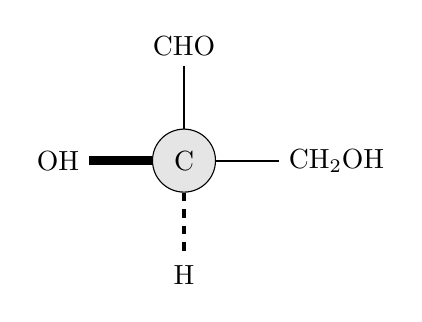
\begin{tikzpicture}[scale=1.0]
  % 3D wedge dash representation of chiral carbon
  \node[circle, draw, fill=gray!20, minimum size=0.8cm] (C) at (0,0) {C};
  \node[above=0.8cm of C] (CHO) {$\ce{CHO}$};
  \node[left=0.8cm of C] (OH) {$\ce{OH}$};
  \node[right=0.8cm of C] (CH2OH) {$\ce{CH2OH}$};
  \node[below=0.8cm of C] (H) {H};
  
  \draw[thick] (C) -- (CHO);
  \draw[line width=3pt] (C) -- (OH); % wedge
  \draw[dashed, line width=1.5pt] (C) -- (H); % dash
  \draw[thick] (C) -- (CH2OH);
\end{tikzpicture}
\end{center}
\begin{enumerate}[label=(\alph*), leftmargin=*]
  \item The four groups attached to the central carbon are: $-\ce{OH}$, $-\ce{CHO}$, $-\ce{CH2OH}$, and $-\ce{H}$.
        Assign priorities 1 and 4 based on the atoms directly attached to the chiral carbon.
  \item The remaining two groups both connect via carbon atoms ($Z=6$), creating a tie.
        The carbon in $-\ce{CHO}$ is double-bonded to oxygen (treated as two bonds to oxygen, so bonded to $(\ce{O}, \ce{O}, \ce{H})$). The carbon in $-\ce{CH2OH}$ is bonded to $(\ce{O}, \ce{H}, \ce{H})$.
        Resolve the tie to assign priorities 2 and 3.
  \item Since H (priority 4) points away (dashed line), trace the direction from 1 $\to$ 2 $\to$ 3. Is the configuration **R** or **S**?
\end{enumerate}
\end{explobox}

\begin{historybox}
\textbf{The Thalidomide Tragedy.}
In the late 1950s, the drug thalidomide was prescribed to pregnant women as a safe sedative to treat morning sickness. The drug was sold as a **racemic mixture** (a 1:1 mixture of both enantiomers). While the (R)-enantiomer acts as an effective sedative, the (S)-enantiomer is a potent teratogen that interferes with blood vessel development in limbs, causing severe birth defects in thousands of children. 
Even if the drug had been prepared as a pure (R)-enantiomer, the disaster would not have been prevented: the human body contains enzymes that catalyze the interconversion (racemization) of the two forms in the bloodstream. This tragedy led to strict international regulations requiring the testing of individual enantiomers of all new chiral drugs.
\{Note: Louis Pasteur's 1848 crystal sorting was the initial milestone that made molecular pharmacology possible.\}
\end{historybox}

\newpage

% ─── Section: Discovery ──────────────────────────────────────────────────────
\section{Part 3 --- Discovery}

\begin{discoverybox}
\textbf{What have we built?}

\textbf{First.} Chirality is a geometric property of asymmetry. A molecule is chiral if it lacks an internal plane of symmetry. A carbon bonded to four different groups is a chiral center.

\textbf{Second.} Enantiomers are non-superimposable mirror images. They share identical physical properties (density, boiling point) but rotate plane-polarized light in opposite directions (optical activity) and interact differently with other chiral environments.

\textbf{Third.} Configurations are named R or S using the Cahn-Ingold-Prelog rules based on atomic number priorities.

\textbf{Fourth.} Diastereomers are stereoisomers that are not mirror images. They have different physical properties and can contain Meso configurations—molecules with chiral centers that are achiral overall due to internal symmetry.
\end{discoverybox}

\newpage

% ─── Section: Naming Concepts ────────────────────────────────────────────────
\section{Part 4 --- What This Is Called}

\begin{namedconcept}{Stereochemical parameters}
* **Chirality:** The geometric property of a molecule that makes it non-superimposable on its mirror image.
* **Enantiomers:** A pair of molecules that are non-superimposable mirror images.
* **Diastereomers:** Stereoisomers that are not mirror images of each other.
* **Meso Compound:** An achiral molecule that contains stereocenters but possesses an internal plane of symmetry.
* **Racemic Mixture:** An optically inactive mixture containing equal amounts of dextrorotatory ($+$) and levorotatory ($-$) enantiomers.
* **Specific Rotation ($[\alpha]_D^T$):** The constant physical property representing the degree of optical rotation of a chemical: $[\alpha] = \alpha / (l \cdot c)$.
\end{namedconcept}

\newpage

% ─── Section: Solved Exercises ───────────────────────────────────────────────
\section{Part 5 --- Solved Exercises}

\begin{problembox}
\begin{enumerate}[label=\textbf{E\arabic*.}]
  \item \textbf{Calculating Stereoisomer Limits.}
  
        Prove that a molecule with $n$ distinct chiral centers can have a maximum of $2^n$ stereoisomers. Explain why this maximum is reduced when meso compounds are present.
        
        \textbf{Solution:}
        Each chiral center can exist in one of two configurations: R or S.
        For a molecule with $n$ independent chiral centers, the configuration of the molecule is a sequence of $n$ choices, where each position in the sequence has 2 possible options:
        \[
          \text{Total Configurations} \;=\; \underbrace{2 \times 2 \times \dots \times 2}_{n \text{ times}} \;=\; 2^n.
        \]
        This represents the maximum possible number of stereoisomers.
        
        However, if the molecule is structurally symmetric, some of these configurations will contain an internal plane of symmetry.
        A configuration with an internal plane of symmetry (a **meso compound**) is superimposable on its own mirror image. This means the R,S and S,R forms of a symmetric molecule are actually the *same* identical molecule:
        \[
          (1R, 2S) \;\equiv\; (1S, 2R) \quad \text{(Meso)}.
        \]
        Because these two configurations represent the same physical molecule, the actual number of unique, isolated stereoisomers is reduced below $2^n$.
        
  \item \textbf{Calculating Enantiomeric Excess.}
  
        A pure enantiomer of a chiral compound has a specific rotation of $[\alpha]_D^{20} = +60.0^\circ$.
        An experimental mixture of this compound and its mirror image is analyzed in a polarimeter tube of length \SI{1.0}{dm} at a concentration of \SI{0.10}{g/mL}. The observed rotation is $+3.60^\circ$.
        Calculate the **enantiomeric excess (ee)** and the percentage of each enantiomer in the mixture.
        
        \textbf{Solution:}
        First, we calculate the specific rotation $[\alpha]_{\text{mix}}$ of our mixture using the formula:
        \[
          [\alpha]_{\text{mix}} \;=\; \frac{\alpha}{l \cdot c},
        \]
        where $\alpha = +3.60^\circ$, $l = 1.0$ dm, and $c = 0.10$ g/mL.
        \[
          [\alpha]_{\text{mix}} \;=\; \frac{+3.60^\circ}{1.0 \times 0.10} \;=\; +36.0^\circ.
        \]
        The enantiomeric excess is the ratio of the mixture's specific rotation to that of the pure enantiomer:
        \[
          \text{ee} \;=\; \frac{[\alpha]_{\text{mix}}}{[\alpha]_{\text{pure}}} \times 100\% \;=\; \frac{+36.0^\circ}{+60.0^\circ} \times 100\% \;=\; 60.0\%.
        \]
        This means $60\%$ of the mixture consists of the pure ($+$)-enantiomer, while the remaining $40\%$ consists of a racemic mixture ($20\%$ ($+$) and $20\%$ ($-$) enantiomers).
        
        Thus, the total percentages are:
        * **Percentage of ($+$)-enantiomer:** $60\% + 20\% = 80\%$.
        * **Percentage of ($-$) -enantiomer:** $20\%$.
\end{enumerate}
\end{problembox}

\newpage

% ─── Section: Problems ───────────────────────────────────────────────────────
\section{Part 6 --- Problems}

\begin{problembox}
\begin{enumerate}[label=\textbf{P\arabic*.}]
  \item \textbf{Tartaric Acid Stereocenters.}
  
        Tartaric acid has the structural formula:
        \[
          \ce{HOOC-CH(OH)-CH(OH)-COOH}.
        \]
        It contains two chiral carbons (C2 and C3).
        \begin{enumerate}[label=(\alph*)]
          \item Draw the Fischer projections for the three stereoisomers: the (2R, 3R) form, the (2S, 3S) form, and the (2R, 3S) form.
          \item Identify which two forms are a pair of enantiomers.
          \item Show why the (2R, 3S) form is a meso compound by locating its internal plane of symmetry. Explain why this compound is optically inactive.
        \end{enumerate}

  \item \textbf{CIP Configuration Naming.}
  
        Determine the R/S configuration of the chiral carbons in the following molecules:
        \begin{enumerate}[label=(\alph*)]
          \item 2-chlorobutane: $\ce{CH3-*CH(Cl)-CH2-CH3}$.
          \item L-alanine (an amino acid):
                \begin{center}
                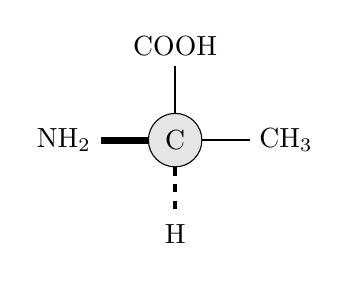
\begin{tikzpicture}[scale=0.8]
                  \node[circle, draw, fill=gray!20] (C) at (0,0) {C};
                  \node[above=0.6cm of C] (COOH) {$\ce{COOH}$};
                  \node[left=0.6cm of C] (NH2) {$\ce{NH2}$};
                  \node[right=0.6cm of C] (CH3) {$\ce{CH3}$};
                  \node[below=0.6cm of C] (H) {H};
                  \draw[thick] (C) -- (COOH);
                  \draw[line width=2.5pt] (C) -- (NH2); % wedge
                  \draw[dashed, line width=1.5pt] (C) -- (H); % dash
                  \draw[thick] (C) -- (CH3);
                \end{tikzpicture}
                \end{center}
        \end{enumerate}
\end{enumerate}
\end{problembox}

\newpage

% ─── Section: Deep Problems ──────────────────────────────────────────────────
\section{Part 7 --- Deep Problems}

\begin{deepbox}
\begin{enumerate}[label=\textbf{D\arabic*.}]
  \item \textbf{The Resolution of Enantiomers.}
  
        Because enantiomers have identical physical properties (boiling point, solubility), they cannot be separated by standard distillation or filtration.
        To separate a racemic mixture of a chiral organic acid ($\pm$-$\ce{A}$), we react it with a pure enantiomer of a chiral amine base, such as natural ($-$) -nicotine:
        \[
          (\pm)\text{-}\ce{A} + (-)\text{-}\ce{B} \;\ce{->}\; \text{Salts}.
        \]
        \begin{enumerate}[label=(\alph*)]
          \item Write down the formulas of the two salts formed in this reaction.
          \item Are these two salts enantiomers or diastereomers of each other?
          \item Explain how the fact that they are diastereomers enables us to separate them using fractional crystallization, and how we can subsequently regenerate the pure chiral acids ($+$)-$\ce{A}$ and ($-$) -$\ce{A}$.
        \end{enumerate}

  \item \textbf{Stereochemical Inversion: The $S_N2$ Mechanism.}
  
        In a nucleophilic substitution reaction of a chiral alkyl halide:
        \[
          \ce{Nu- + R-X -> R-Nu + X-}.
        \]
        If the reaction proceeds via the **$S_N2$ mechanism**, the nucleophile attacks the chiral carbon from the side opposite to the leaving group (backside attack).
        \begin{enumerate}[label=(\alph*)]
          \item Sketch the transition state of this backside attack, showing how the three non-reacting groups attached to the chiral carbon are pushed through a planar configuration (like an umbrella turning inside out in the wind).
          \item Explain why this backside attack forces a complete inversion of the spatial configuration at the chiral center. (If the starting material is pure (R), why does the product take the (S) configuration?)
          \item If the reaction proceeded via the **$S_N1$ mechanism** (where the leaving group departs first to form a planar carbocation intermediate $\ce{R+}$), what would be the stereochemical configuration of the product? Why would it lead to a racemic mixture?
        \end{enumerate}
\end{enumerate}
\end{deepbox}

\newpage

% ─── Section: Reflection ─────────────────────────────────────────────────────
\section{Part 8 --- Reflection}

\begin{reflectionbox}
\textbf{Conceptual Reflection}

Consider the following questions:
\begin{enumerate}
  \item **On the Origin of Homochirality:** All living organisms on Earth use exclusively L-amino acids to build proteins and D-sugars for DNA. Enantiomers are thermodynamically identical in energy. Why did life choose one hand over the other? Was it a random frozen accident in the prebiotic soup, or is there a physical asymmetry (such as the weak nuclear force violating parity) that favors one hand?
  \item **On Drug Design:** The active sites of enzymes are chiral pockets made of L-amino acids. Why does this explain why one enantiomer of a drug fits like a key in a lock, while its mirror image does not fit at all, or fits into other receptors causing toxicity?
  \item **On Pasteur's Insight:** Pasteur stated: "Life is dominated by asymmetric actions. I can foresee that all living species are primordially, in their structure, in their external forms, functions of cosmic asymmetry." What did he mean by this?
\end{enumerate}
\end{reflectionbox}

\medskip
\noindent\textbf{Looking ahead.}
Module~6.3 introduces **Resonance and Aromatics**. Having explored spatial geometries and configurations, we will investigate how electrons behave when they are not locked into single or double bonds, but are free to delocalize across entire ring structures. We will study Hückel's rule and the unique stability of benzene.

\vspace{1.4cm}
\begin{center}
{\color{JourneyColor}\rule{0.5\linewidth}{0.8pt}}\\[6pt]
{\small\color{JourneyColor}\textit{End of Journey 6, Module 6.2 --- Isomerism and Stereochemistry}}\\[4pt]
{\small\color{JourneyColor}Continue to: \textbf{Module 6.3 --- Resonance and Aromatics}}\\[6pt]
{\color{JourneyColor}\rule{0.5\linewidth}{0.8pt}}
\end{center}

\end{document}
